\section{Synteny}

\subsection{Methods}

\subsubsection{Macrosynteny}
\textcolor{red}{pipeline}

\subsubsection{Microsynteny}
\textcolor{red}{Synchro}

\subsection{Results}

\subsubsection{Genome Assembly Analysis}

\textcolor{red}{TODO: number of scaffolds, number of genes, distribution of scaffold sizes (MB, genes)}

\subsubsection{Phylogeny Tree}

\subsubsection{Macrosynteny}

\begin{figure}[h!]
  \centering
    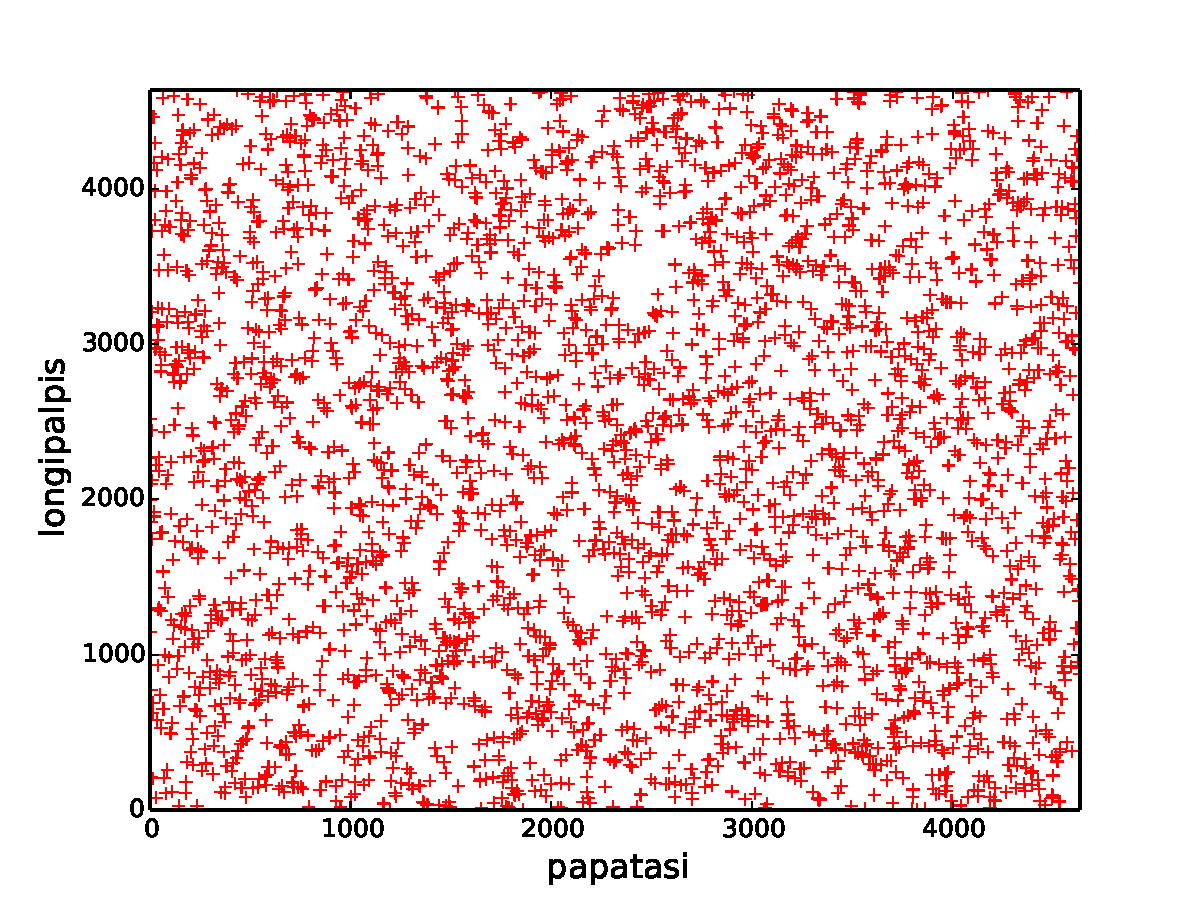
\includegraphics[width=0.8\textwidth]{figures/synteny/papatasi_longipalpis_plot}
  \caption{Locations of homologous genes in \emph{L. longipalpis} and \emph{P. papatasi}}
\end{figure}

\begin{figure}[h!]
  \centering
    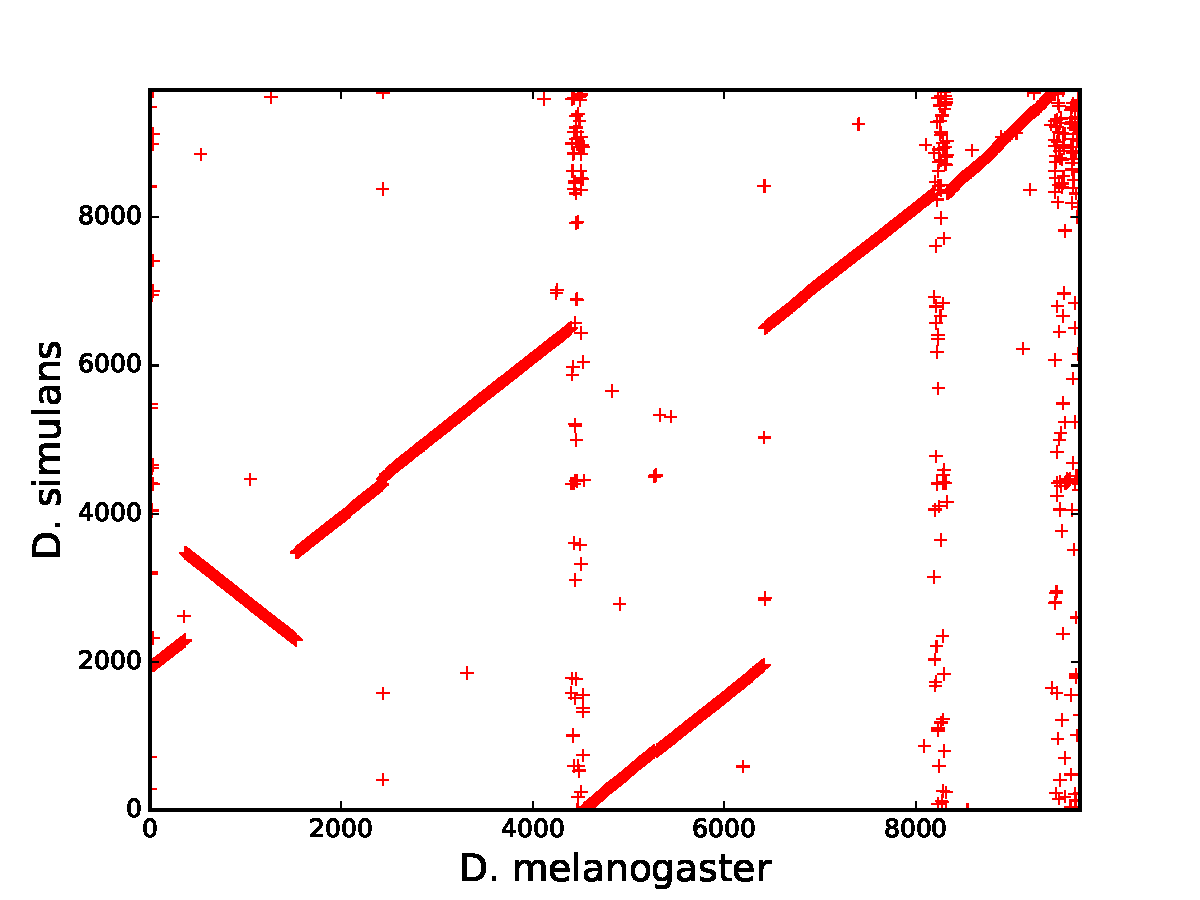
\includegraphics[width=0.8\textwidth]{figures/synteny/dmel_dsim_plot}
  \caption{Locations of homologous genes in \emph{D. melanogaster} and \emph{D. simulans}}
\end{figure}

\begin{figure}[h!]
  \centering
    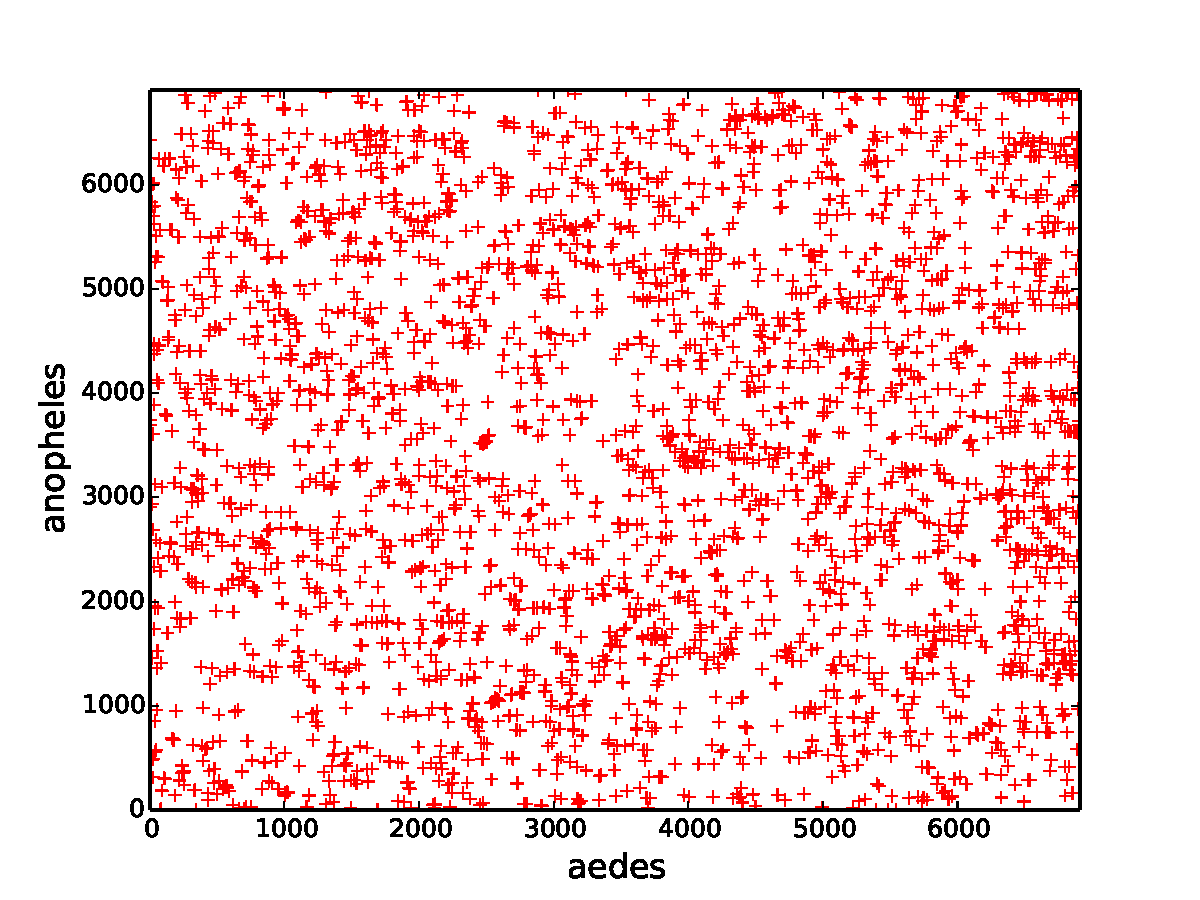
\includegraphics[width=0.8\textwidth]{figures/synteny/aedes_anopheles_plot}
  \caption{Locations of homologous genes in \emph{Ae. aegypti} and \emph{A. gambiae}}
\end{figure}

\begin{figure}[h!]
  \centering
    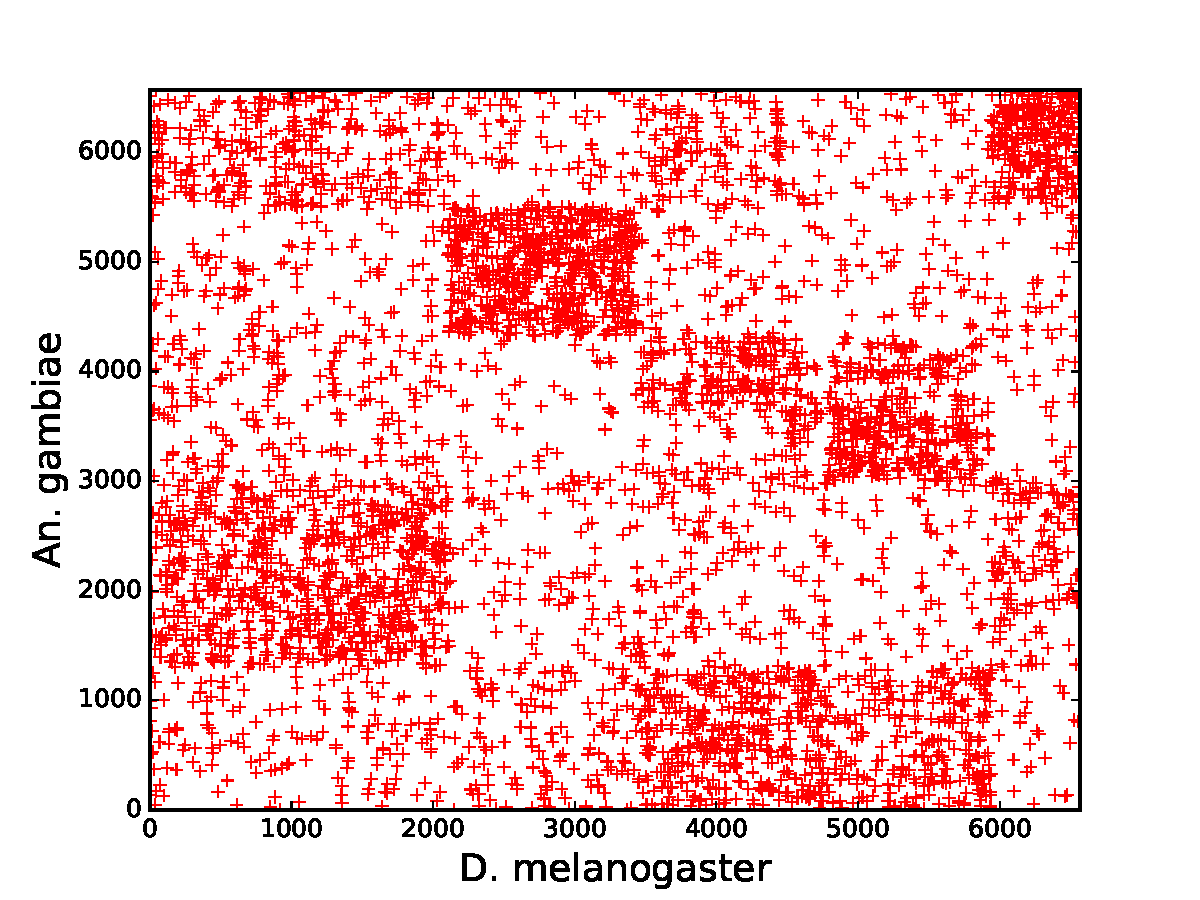
\includegraphics[width=0.8\textwidth]{figures/synteny/dmel_anopheles_plot}
  \caption{Locations of homologous genes in \emph{A. gambiae} and \emph{D. melanogaster}}
\end{figure}

\subsubsection{Microsynteny}

\textcolor{red}{block size distributions}

\textcolor{red}{analysis of individual blocks}

\subsection{Discussion and Conclusion}